\documentclass[11pt,a4paper,oneside]{article}
\usepackage[hangul]{kotex}
\usepackage{olymp}
\usepackage{graphicx}
\usepackage{subcaption}
\usepackage{enumitem}
\usepackage{amsmath}
\usepackage[english]{babel}
\usepackage{amssymb}
\usepackage{import}
\usepackage{multirow}
\usepackage{xcolor}
\usepackage{minted}

% 키파: XeLaTeX 혹은 LuaLaTeX로 컴파일한 뒤 아래 두 줄을 주석해제하면 오류 없이 얼추 비슷한 결과를 얻습니다. 오류 확인을 원할 때 사용하세요.
% \usepackage{fontspec}
% \setmainhangulfont{NanumMyeongjo}

\usepackage{tikz}
\usepackage{pdfpages}


\definecolor{boj}{RGB}{0,118,191}
\definecolor{ucpc-orange}{RGB}{255,153,0}
\definecolor{acgreen}{RGB}{0,159,107}
\definecolor{wared}{RGB}{231,76,60}

\definecolor{acbronze}{RGB}{173,86,0}
\definecolor{acsilver}{RGB}{67,95,122}
\definecolor{acgold}{RGB}{236,154,0}
\definecolor{acplatinum}{RGB}{39,226,164}
\definecolor{acdiamond}{RGB}{0,180,252}
\definecolor{acruby}{RGB}{255,0,98}

%\renewcommand{\baselinestretch}{1.0}

\contest{2025 Soongsil Programming Contest}{SCCC@SoongsilU, Sponsors: Startlink, Channel Corporation, HANBIT MEDIA}{May 17th, 2025}

\begin{document}

    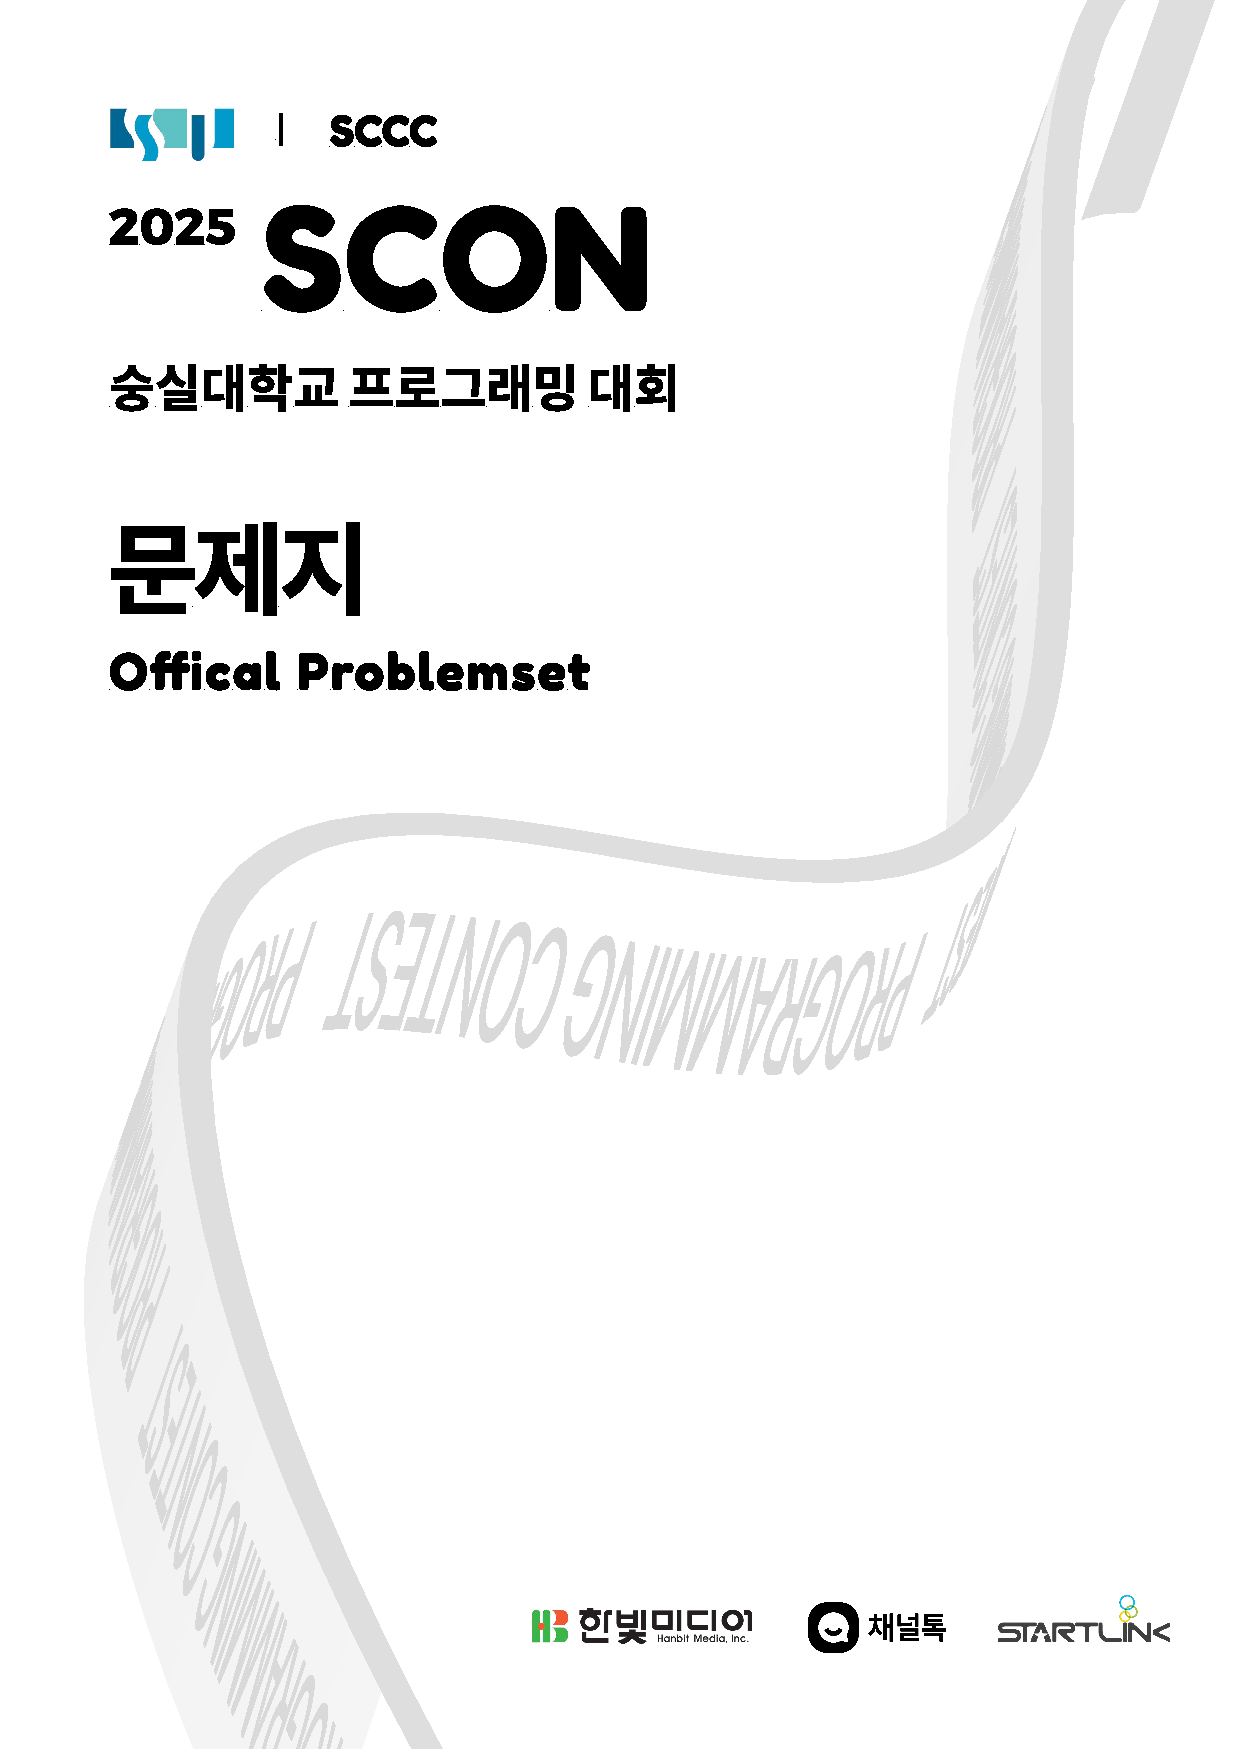
\includepdf[page=1,offset=25mm -38mm]{cover-2025scon.pdf}
%
    \import{./}{language.tex} \pagebreak
    \import{./}{rule.tex} \pagebreak
%
    \begin{center}
    
    \vspace*{15mm}
    {
        \Huge
        \textbf{2025 Soongsil Programming Contest}
        
        \vspace{25mm}
        Problem List
        \vspace{10mm}
    }
    
    \begin{tabular}{|c|l|r|r|r|}
    \hline
    \# & Problem Name & Time limit & Memory limit & Page \\ \hline
        A & 알파벳 블록 & 1 second\phantom{s} & 1024MiB & \phantom{0}8 -- \phantom{0}8 \\ \hline
        B & 합의 최소 & 2 seconds & 1024MiB & \phantom{0}9 -- \phantom{0}9 \\ \hline
        C & 특별상 눈치게임 & 1 second\phantom{s} & 1024MiB & 10 -- 11 \\ \hline
        D & $N$거리 건너기 & 1 second\phantom{s} & 1024MiB & 12 -- 13 \\ \hline
        E & even하게 익은 scon & 1 second\phantom{s} & 1024MiB & 14 -- 14 \\ \hline
        F & A = B $\oplus$ C & 1 second\phantom{s} & 1024MiB & 15 -- 15 \\ \hline
        G & 불꽃놀이의 아름다움 2 & 1 second\phantom{s} & 1024MiB & 16 -- 17 \\ \hline
        H & 서로소 조합 & 1 second\phantom{s} & 1024MiB & 18 -- 18 \\ \hline
        I & 대결 & 1 second\phantom{s} & 1024MiB & 19 -- 20 \\ \hline
        J & 맛있는 스콘 만들기 & 3 seconds & 1024MiB & 21 -- 22 \\ \hline
    \end{tabular}

    \vspace{5mm}
    
    문제지에 있는 문제가 총 10문제가 맞는지 확인하시길 바랍니다.

    문제는 출제진이 생각하는 난이도순으로 정렬되어 있지만, 모든 문제를 읽고 고민하는 것을 권장합니다.

    모든 문제는 C++17, Java 15, PyPy3으로 풀 수 있음을 보장합니다. (단, Python 3는 보장하지 않음)
    
    \end{center}
    	
    \pagebreak

    \import{2025/alphabet-block/}{main.tex} \pagebreak
    \import{2025/seq-min-sum/}{main.tex} \pagebreak
    \import{2025/prize-game/}{main.tex} \pagebreak
    \import{2025/n-way-intersection/}{main.tex} \pagebreak
    \import{2025/even-sccc-scon/}{main.tex} \pagebreak
    \import{2025/xor/}{main.tex} \pagebreak
    \import{2025/coloring/}{main.tex} \pagebreak
    \import{2025/coprime-combination/}{main.tex} \pagebreak
    \import{2025/divide-team/}{main.tex} \pagebreak
    \import{2025/delicious-scon/}{main.tex} \pagebreak
    
\end{document}